\section{Análisis}
\label{section:analisis}

\subsection{El mundo}
Siendo el objetivo principal del proyecto crear un banco de pruebas para la medición del estrés en manadas de entidades autónomas por medio del sistema auditivo, reproduciremos el modelo propuesto por Craig W. Reynolds en su trabajo “Steering Behaviors For Autonomous Characters” para la creación de dichos agentes autónomos.
 
Para que las entidades puedan existir es necesario crear previamente un espacio con ciertas características donde puedan cohabitar grupos de dichas entidades.
 
Para ello, se creará un mundo en dos dimensiones (x,y) con una perspectiva de planta para su representación gráfica. La coordenada (0,0) se situará en la esquina superior izquierda del canvas.
 
El mundo contará con un tiempo inicial y actual, esta magnitud medible es necesaria para el correcto funcionamiento del sistema. Con ella la velocidad máxima de ciclos de procesamiento dependerá del aumento del tiempo y no de la velocidad propia que pueda alcanzar el procesador principal del sistema. Esto es de suma importancia porque proporciona una independencia a la hora de ejecutar la aplicación en diferentes sistemas con diferentes capacidades de calculo.
 
Dispondrá de un largo y ancho para su representación gráfica pero en la práctica y a la hora de realizar cálculos no tendrá ninguna limitación de tamaño, esto permite una gran libertad a la hora de realizar diferentes comportamientos por las entidades, la representación gráfica solo es una ventana donde poder observar todo lo que ocurre en el sistema.
 
Se podrán marcar algunas reglas físicas para adecuar el mundo virtual al real o caracterizarlo de cierta manera. Se podrá acotar la velocidad máxima y la aceleración máxima que pueden alcanzar las entidades, entre otras cosas.
 
El mundo dispondrá de una lista de todas las entidades y objetos que se encuentren dentro del mismo. Gracias a esto, será más fácil el cálculo y programación de comportamientos, además de, para labores de optimización de la aplicación.
 
Los objetos u obstáculos se definirán con líneas rectas y se podrán formar figuras geométricas con ellas.  Esto da la posibilidad desde crear recintos para acotar el espacio de movimiento a crear obstáculos para definir caminos o simplemente para que sean evitados.
 
\subsection{Nanobot}
\label{sec:nanobot}

Cada nanobot sera una entidad que percibe su entorno y que podrá ser capaz de actuar en consecuencia decidiendo que hacer por medio de unas reglas de logica propias del modelo[Figura \ref{fig:../images/procesoNanobot.png}].
\begin{figure}[h]
 \centering
 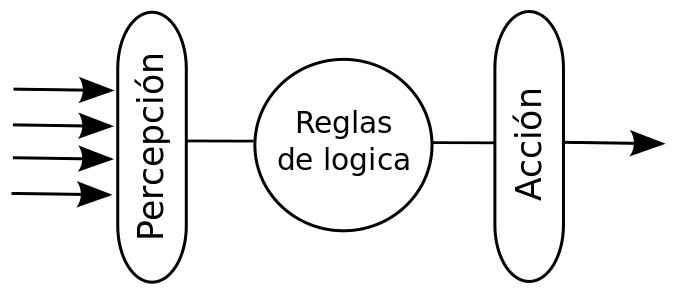
\includegraphics[scale=0.3]{../images/procesoNanobot.png}
 % procesoNanobot.png: 676x294 pixel, 72dpi, 23.85x10.37 cm, bb=0 0 676 294
 \caption{Proceso de la toma de decisiones de las entidades}
 \label{fig:../images/procesoNanobot.png}
\end{figure}

Gracias a esto cada nanobot del grupo poseerá cierto nivel de inteligencia, sera capaz de actuar de manera autónoma y  tener un nivel complejo de predictibilidad  a largo plazo. Al no tratarse de un sistema ideal toda la información que le llegue sera acotada para simular un entorno real, es decir, tanto su sistema visual y auditivo serán finitos y acordes a los animales que representen.

\subsubsection{Características básicas}
\label{sec:caracteristicas_basicas}

\noindent Las principales características de los Nanobots son:  
\begin{itemize}
 \item  Cerebro: En el cerebro se gestionan todos los comportamientos. Se dispondrá de una lista de la cual se podrá elegir el comportamiento adecuado en cada momento para el correcto funcionamiento del modelo. También se podrán activar mas de un comportamiento dando lugar a otros comportamientos mas complejos e impredecibles. Sera capaz de saber cual es la aceleración adecuada para poder variar la velocidad de manera correcta. Esto se realizara haciendo la media de todas las aceleraciones devueltas por los comportamientos y en función de esa aceleración la velocidad de la entidad se adecuara a la situación actual.
 \item Geo data: Se debe conocer en todo momento la posición del nanobot, así como, su velocidad y aceleración. Imprescindible para poder realizar todos los cálculos de los comportamientos y de su representación gráfica. Estas tres magnitudes serán representadas por vectores de dos dimensiones al igual que el mundo.
 \item Masa: Es la cantidad de materia que posee cada entidad. Necesaria para calcular la inercia mecánica del móvil. 
 \item Visión: Define el ángulo y radio de visión. Con ello se podrá calcular todas las entidades que son susceptibles a ser vistas.
 \item Dirección: Con ella se podrá determinar la dirección en la que mira el nanobot, será calculada como el vector unitario del vector velocidad.
 \item Límites de la fuerzas: Cada entidad poseerá unos límites físicos para la correcta simulación del modelo, se busca con estos límites dotar de realismo a la simulación [Figura \ref{fig:../images/fuerzas_limite.png}]. 
 Estos limites son:
 \begin{itemize}
   \item Aceleración: Sólo sera posible una aceleración máxima. Superada esa aceleración se volverá inmediatamente a la aceleración máxima.
   \item Giro: Determina el ángulo máximo de giro.
   \item Frenado: Máxima fuerza de frenado que podrá ejercer el nanobot. 
 \end{itemize}	
\begin{figure}[h]
 \centering
 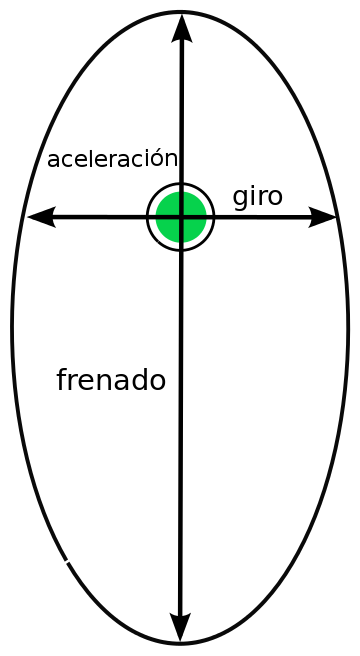
\includegraphics[scale=0.3]{../images/fuerzas_limite.png}
 % fuerzas_limite.png: 360x656 pixel, 90dpi, 10.16x18.52 cm, bb=0 0 288 525
 \caption{Esquema de las fuerzas límite.}
 \label{fig:../images/fuerzas_limite.png}
\end{figure}
 \item Velocidad máxima: En todo momento se debe revisar el valor de la velocidad, si el módulo del vector velocidad es mayor que la velocidad máxima impuesta, esta se reducirá inmediatamente.
 \item Nivel de estrés: Se dispone de un sistema para medir el estrés del sujeto. Con él, se podrá definir un nivel de estrés en función de todo lo que escuche, desde musica a otros nanobots.
 \item Distancia que recorre la onda de sonido: al poder producir sonido, se define una distancia máxima a la que el sonido producido puede llegar.
\end{itemize}




\subsubsection{Visión}
\label{sec:vision}

Cada entidad posee un campo de visión que esta determinado por un radio de visión y un ángulo[Figura \ref{fig:../images/angulo_vision.png}]. Estos dos valores podrán ser parametrizados para observar diferentes reacciones y comportamientos. 

Para la obtención de las entidades locales que es capaz de visualizar se realizara una resta de los vectores de posición desde el origen de coordenadas de cada integrante del mundo con respecto al observador, si la distancia es menor al radio de visión es un objeto o entidad susceptible a ser observada , para asegurarlo se realizara además una segunda comprobación con respecto al ángulo que forma con la otra entidad, si este  es menor al ángulo de visión es un objeto que es visualizado por la entidad.

\begin{figure}[h]
 \centering
 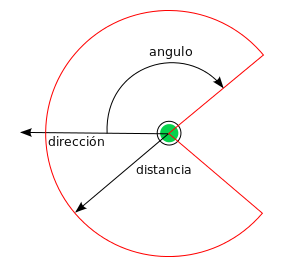
\includegraphics[scale=0.7]{../images/angulo_vision.png}
 % angulo_vision.png: 304x267 pixel, 90dpi, 8.58x7.54 cm, bb=0 0 243 214
 \caption{Visión.}
 \label{fig:../images/angulo_vision.png}
\end{figure}


\subsubsection{Audición}
\label{sec:audicion}

Cada entidad poseerá un sistema auditivo que hará posible el sentido del oído, es decir, lo faculta para ser sensible a los sonidos. La función principal de esto sera transformar las ondas sonoras que se propagan por el aire en información que capta la entidad y transmite al cerebro para su procesamiento y posterior reacción.


\subsubsection{Sistema de comportamientos}
\label{sec:sistema_comportamientos}

La principal regla en el sistema de comportamientos se basa en la ausencia de una inteligencia que domine a todas las entidades o sobresalga del grupo. Lo contrario invalida el modelo computacional y lo hace carente de sentido para su estudio. Al tener todos los nanobots un nivel similar de inteligencia ayuda a la hora de calcular, estudiar y medir los patrones de bandadas que pueden llegar a formar con las diferentes  ponderaciones que se pueden realizar a sus atributos básicos. Siendo este el motivo principal de estudio del presente proyecto.\\

\noindent\textbf{Comportamientos de manada}

Son las reglas básicas por las que entidades independientes se comportarán de manera similar a manadas de animales reales. Estas reglas son:
\begin{itemize}
 \item Alineación: Se busca que todas las entidades tengan una dirección común. Para ello, se obtiene la velocidad de todas las entidades vecinas y se calcula su promedio, dicho promedio será la velocidad deseada[Figura 5].
 
  \begin{figure}[h]
 \centering
 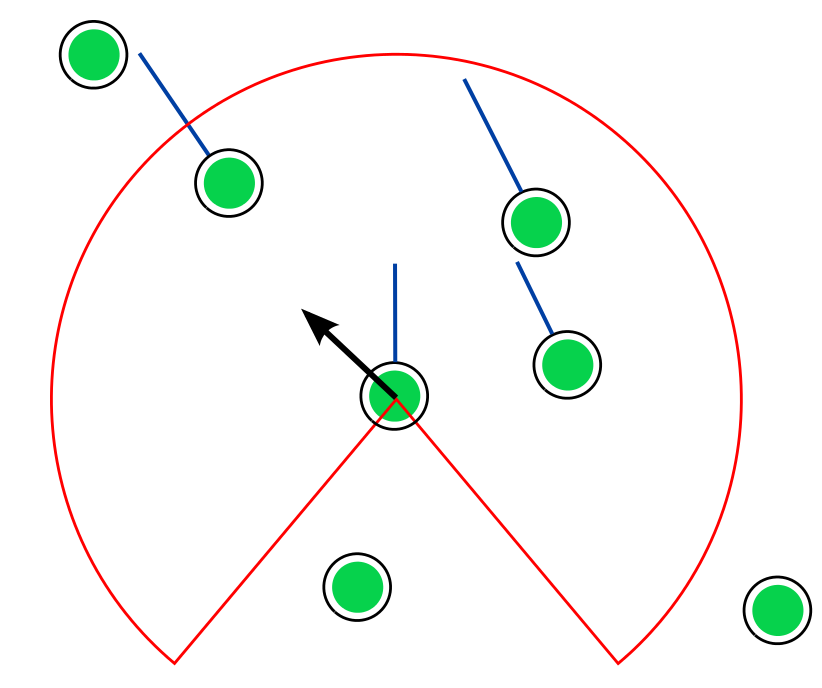
\includegraphics[scale=0.2]{../images/alineacion.png}
 \caption{Alineación.}
 \label{fig:../images/flee.png}
 \end{figure}
 
 \item Cohesión: Las entidades se mantienen unidas, es decir, se busca que los nanobots no se separen con respecto a una distancia máxima. Para ello, se buscan las posiciones de las entidades vecinas y el promedio de esas posiciones sera el punto que seguirá cada nanobot para mantener la unidad [Figura 6].
 
   \begin{figure}[h]
 \centering
 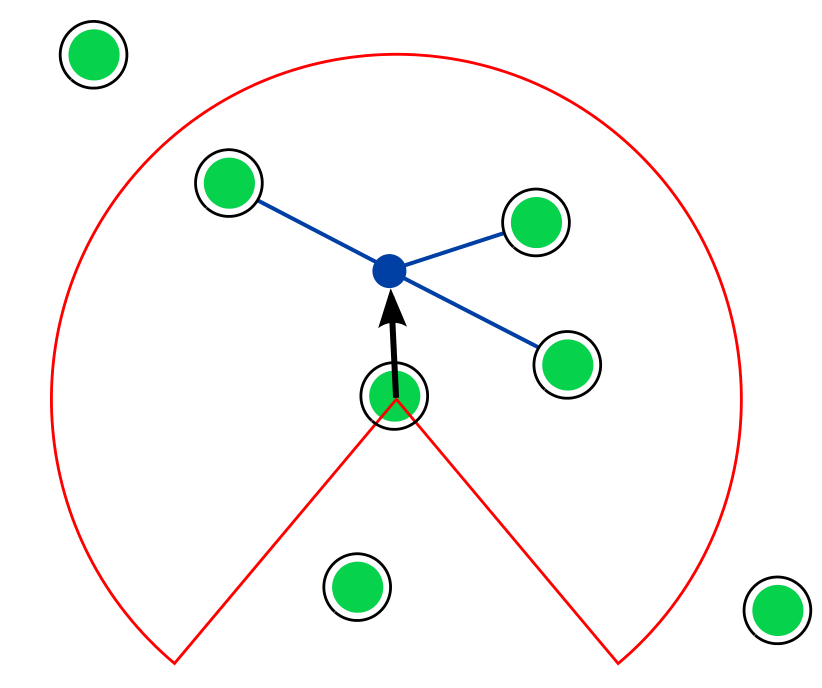
\includegraphics[scale=0.2]{../images/cohesion.png}
 \caption{Cohesión.}
 \label{fig:../images/flee.png}
 \end{figure}
 
 \item Separación: Las entidades buscan una separación mínima con su vecinas. Por eso se busca la distancia de separación de las entidades con respecto al observador. Mientras esa distancia sea grande la fuerza de repulsión sera pequeña y viceversa, a una distancia muy pequeña la fuerza sera muy grande [Figura 7].

   \begin{figure}[h]
 \centering
 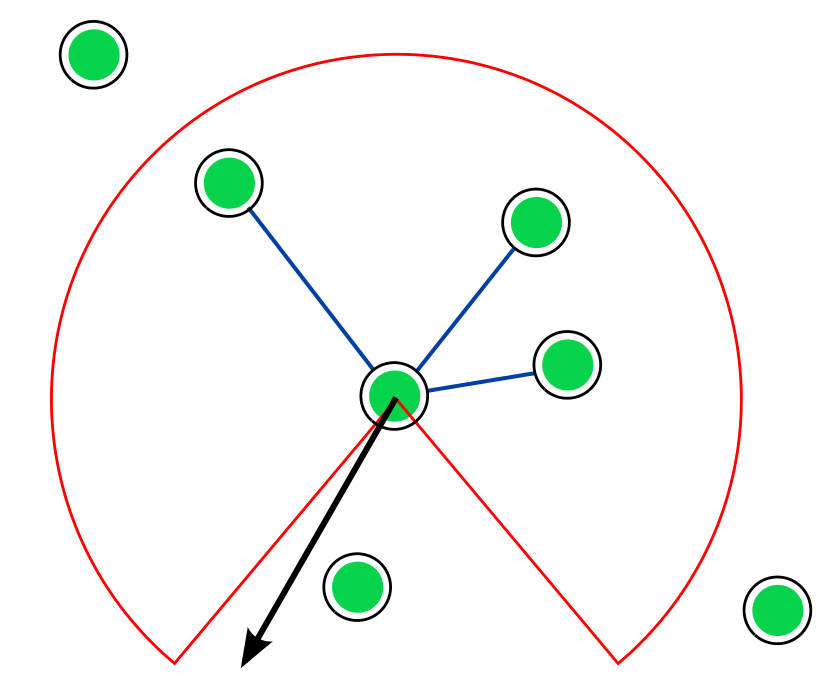
\includegraphics[scale=0.2]{../images/separation.png}
 \caption{Separación.}
 \label{fig:../images/flee.png}
 \end{figure}
 
 \end{itemize}

\paragraph{Comportamientos individuales}
Se basan en acciones específicas para cada entidad en particular, son:  
\begin{itemize}
 \item Seguir: El nanobot buscará la última posición en la que se encuentre su objetivo. Se calculará una velocidad deseada que será el resultado de escalar el vector unitario de la distancia entre perseguidor y objetivo por la velocidad máxima. Para posteriormente calcular la aceleración deseada restando a la velocidad deseada la velocidad actual [Figura 8]. 
 
 \begin{figure}[H]
 \centering
 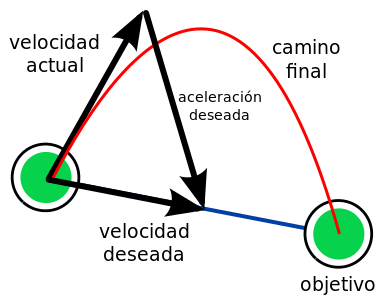
\includegraphics[scale=0.4]{../images/seek.png}
 \caption{Seguir.}
 \label{fig:../images/seek.png}
 \end{figure}

\item Alejarse: Se trata del comportamiento inverso a seguir. Se realizará el mismo cálculo pero al resultado se le cambiara el signo [Figura 9]. 

 \begin{figure}[H]
 \centering
 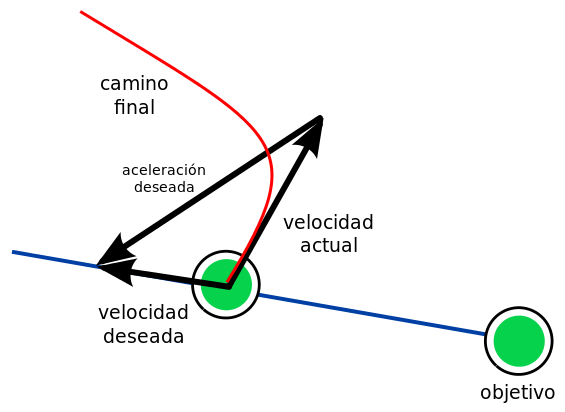
\includegraphics[scale=0.4]{../images/flee.png}
 \caption{Alejarse.}
 \label{fig:../images/flee.png}
 \end{figure}

\item Perseguir: El nanobot buscará una futura posición en el tiempo en la que se encuentre su objetivo. Se calculará una velocidad deseada que será el resultado de escalar el vector unitario de la distancia entre perseguidor y la posición futura del objetivo por la velocidad máxima. Para posteriormente calcular la aceleración deseada restando a la velocidad deseada la velocidad actual [Figura 10].

 \begin{figure}[H]
 \centering
 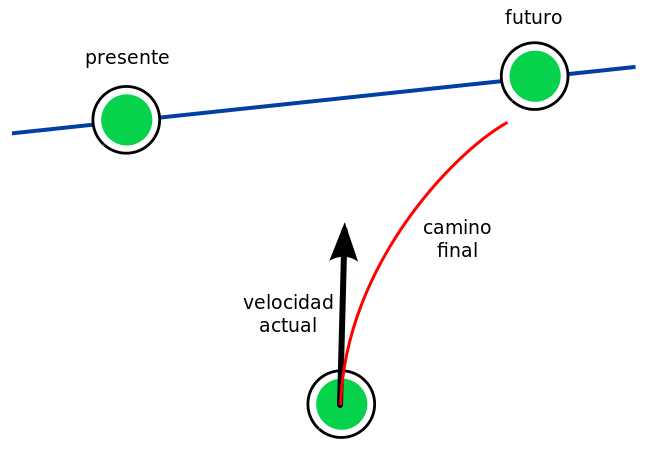
\includegraphics[scale=0.4]{../images/pursuit.png}
 \caption{Perseguir.}
 \label{fig:../images/pursuit.png}
 \end{figure}

 \item Huir: Se trata del comportamiento inverso a perseguir. Se realizará el mismo cálculo pero al resultado se le cambiara el signo [Figura 11]\\. 
% \item Perseguir: El nanobot buscará una futura posición en el tiempo en la que se encuentre su objetivo. Se calculará una velocidad deseada que será el resultado de escalar el vector unitario de la distancia entre perseguidor y la posición futura del objetivo por la velocidad máxima. Para posteriormente calcular la aceleración deseada restando a la velocidad deseada la velocidad actual [Figura 8].


 \begin{figure}[H]
 \centering
 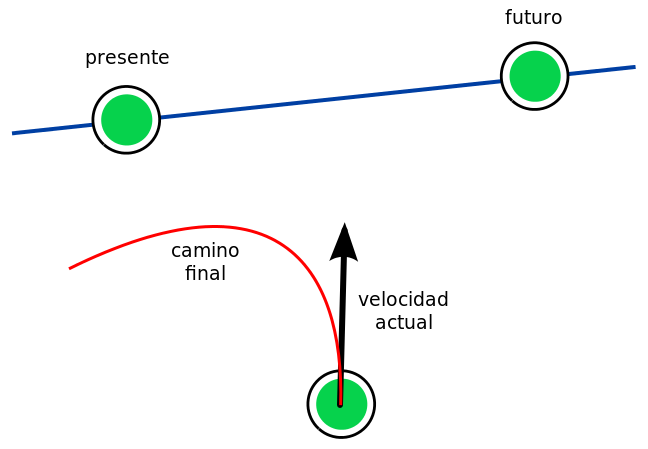
\includegraphics[scale=0.4]{../images/evasion.png}
 \caption{Huir.}
 \label{fig:../images/evasion.png}
 \end{figure}

\item Evitar obstáculos: Cada nanobot será capaz de evitar obstáculos que se encuentre en su camino. Para ello, se creará una línea imaginaria que es idéntica al vector velocidad que lleve en ese momento. Si esa línea imaginaria intersecta con cualquier línea que esté definida en el mundo para crear obstáculos, la aceleración deseada será el vector normal a la velocidad [Figura 12]. \\

\begin{figure}[H]
 \centering
 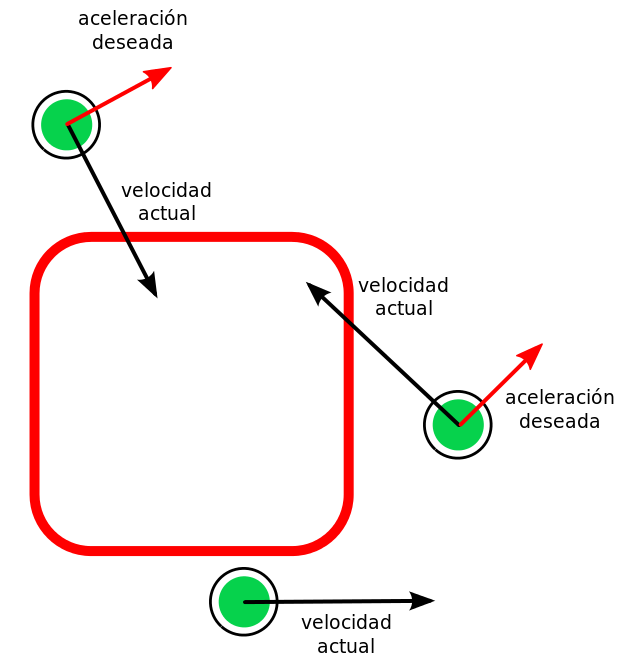
\includegraphics[scale=0.4]{../images/containment.png}
 \caption{Evitar obstáculos.}
 \label{fig:../images/containment.png}
 \end{figure}

 \item Vagar: Permite a los nanobots vagar libremente por el mundo sin un rumbo fijo y sin dar cambios bruscos de dirección. Se calculará una velocidad deseada que será el resultado de escalar el vector unitario de la distancia entre el nanobot y  un punto aleatorio  por la velocidad máxima. Para posteriormente calcular la aceleración deseada restando a la velocidad deseada la velocidad actual [Figura 13].  

  \begin{figure}[h]
 \centering
 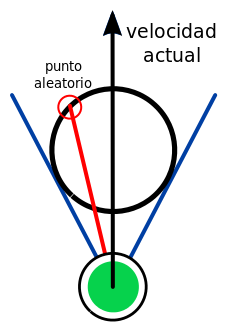
\includegraphics[scale=0.4]{../images/wander.png}
 \caption{Vagar.}
 \label{fig:../images/wander.png}
 \end{figure}
 
 \end{itemize}


\subsubsection{Toma de decisiones}
\label{sec:toma_decisiones}
La aplicación de cada uno de los comportamientos nos indicará hacia donde se debe dirigir el nanobot, al darse la posibilidad de tener activados tantos comportamientos como se deseen o necesiten, la toma de decisión que se realizará será la media de la suma de cada uno de los comportamientos, dando como resultado una aceleración vectorial que influirá en la velocidad de la entidad [Figura 14].

 \begin{figure}[h]
 \centering
 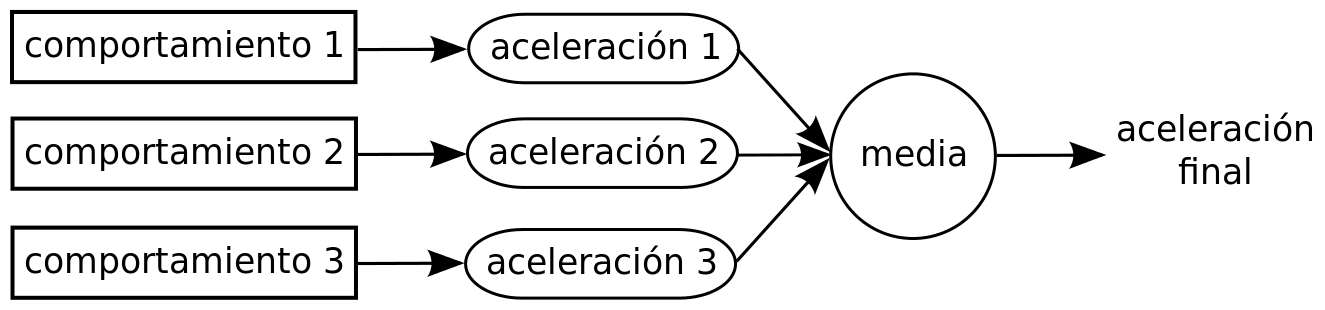
\includegraphics[scale=0.3]{../images/toma_decisiones.png}
 \caption{Toma de decisiones.}
 \label{fig:../images/toma_decisiones.png}
 \end{figure}

\subsubsection{Comunicación oral}
\label{sec:comunicacion_oral}

Cada entidad será capaz de comunicarse con sus semejantes en un determinado radio.  Cada nanobot podrá mandar mensajes, siendo así el emisor, susceptibles a ser recibidos por todos los nanobot que se encuentre en el radio de la onda sonora, convirtiéndolos en los receptores del mensaje. Se debe diferenciar el receptor del emisor para que al responder no se produzca un efecto en cadena si otro está escuchando.

Existen dos tipos diferentes de comunicaciones:
\begin{itemize}
 \item Comunicación simple: Donde solo se intercambian palabras para poder modificar de manera muy rápida el nivel de estrés del receptor. No hay posibilidad de una segunda réplica por parte del emisor. 
 \item Comunicación ligada a una orden: Se trata de comunicar una orden directa a todas los nanobots que estén escuchando. Estas entidades la procesaran y la llevaran a cabo inmediatamente después.  
\end{itemize}

De esta forma estarán capacitados para poder comunicarse de una manera simple. 

\subsubsection{Nivel de estrés}
\label{sec:nivel_estres}
Cada nanobot poseerá un nivel de estrés para reaccionar de acuerdo a el. Según el nivel de estrés  ciertos valores básicos del nanobot cambiaran. Los valores susceptibles a ser modificados son:  ángulo de visión, capacidad de giro, frenado, aceleración y velocidad máxima. 

\subsection{Speaker}
\label{sec:speaker}
Un speaker, o altavoz, es la simulación de un transductor electroacústico que se utiliza para la reproducción de sonido. Cada speaker es capaz de reproducir canciones de una lista de reproducción, estas canciones serán analizadas a la hora de ser reproducidas. Todas las entidades que escuchen al speaker recibirán la frecuencia del sonido y la interpretaran según sea conveniente.
 
Un speaker será capaz de estar, o no, encendido. Al encenderlo se reproducirá la canción que este actualmente seleccionada, existiendo además una opción para poder pasar a la siguiente canción.
 
También se podrá aumentar, o disminuir, el volumen general del speaker. Con ello variará, no sólo, el volumen de la canción, sino también el radio de alcance de la onda sonora. Con esto se podrá crear diferentes zonas de influencia de la música, con todas las posibilidades de experimentación que ello conlleva.


\subsection{AudioContext}
\label{sec:audio_context}
La idea de esta API de alto nivel, para poder procesar y sintetizar audio en aplicaciones Web se basa en el concepto de nodos de audio (AudioNode), que serán los elementos que se interconectarán entre sí para formar una cadena, cuyo resultado será el audio renderizado. Lo primero que deberemos definir es un contexto para estos nodos, donde se producirán todos los sonidos. Puede soportar varias fuentes de audio, con lo que sólo necesitaremos un contexto por cada aplicación de audio.

La forma de crear el contexto sería así:
\begin{verbatim}
var context;\end{minipage}
window.addEventListener('load', init, false);

function init() {
  try {
    window.AudioContext = window.AudioContext||
                          window.webkitAudioContext||
                          window.mozAudioContext||
                          window.oAudioContext||
                          window.msAudioContext;
    context = new AudioContext();
  } catch(e) {
    alert('Este navegador no soporta la API de audio');
  }
}
\end{verbatim}

Esta instancia del contexto  permite acceder a un montón de métodos para crear nodos de audio, o manejar las preferencias globales de audio. Se centrará la atención en los nodos de audio, ya que son elementos necesarios en la cadena anteriormente citada.

Web Audio API cuenta con ruteo modular: Se puede ir ruteando las señales, a través de arquitecturas simples o complejas, que pasen por envíos y retornos, por ejemplo a efectos, mezclas y submezclas, …\\

Existen nodos de varios tipos:
\begin{itemize}
 \item Nodos de origen: fuentes de sonido, buffers de audio, entradas de sonido en vivo, $<$audio$>$tags, osciladores, y procesadores JS.
 \item Nodos de modificación: como su propio nombre indica sirven para modificar el sonido: filtros, paneadores, procesadores JS, convoluciones,…
 \item Nodos de destino: las salidas de audio.
\end{itemize}

Por tanto, para generar una cadena de audio, se debe generar los orígenes,  los modificadores, los destinos, y se conectarán todos a través del método connect(). De la misma forma se podrán  desconectar con el método disconect (numeroPuertoSalida), y volverlos a conectar.  En resumen:  Se pueden crear las cadenas de forma dinámica.

\begin{verbatim}
 // Creamos un nodo origen
 var origen = context.createBufferSource();
 // Creamos un nodo modificador en este caso un Gain node
 var gain = context.createGain();
 // Conectamos el origen con el modificador
 origen.connect(gain);
 // Conectamos el modificador con el destino por defecto del contexto
 gain.connect(context.destination);

 // desconectamos el origen
 origen.disconnect(0);
 // Desconectamos el modificador
 gain.disconnect(0);
 // Conectamos directamente el origen al destino por defecto del contexto
 origen.connect(context.destination);
\end{verbatim}

\subsection{Cómo cargar sonidos}
\label{sec:cargar_sonidos}
La Web Audio API utiliza un AudioBuffer para sonidos de duración media-corta. El enfoque básico es usar una llamada XMLHttpRequest para ir a buscar los archivos de sonido. 
El API es compatible con la carga de datos de los archivos de audio en múltiples formatos, como WAV, MP3, AAC, OGG y otros.\\

El siguiente fragmento muestra la carga una muestra de sonido:
\begin{verbatim}
 var dogBarkingBuffer = null;
 window.AudioContext = window.AudioContext || window.webkitAudioContext;
 var context = new AudioContext();

 function loadDogSound(url) {
  var request = new XMLHttpRequest();
  request.open('GET', url, true);
  request.responseType = 'arraybuffer';

  request.onload = function() {
    context.decodeAudioData(request.response, function(buffer) {
      dogBarkingBuffer = buffer;
    }, onError);
  }
  request.send();
 }
\end{verbatim}

Un buffer no son más que datos en memoria. En este caso, datos que representan un sonido.
Los datos del archivo de audio son binarios (no de texto), por lo que establece la responseType de la solicitud de 'ArrayBuffer'.\\

\noindent\textbf{Para obtener ese buffer}\\
Una vez que los datos de archivo de audio han sido recibidos (sin decodificar), se puede decidir decodificarlos más adelante o inmediatamente, utilizando el método decodeAudioData. Este método toma el ArrayBuffer de datos de archivos de audio almacenados en request.response y los decodifica de forma asíncrona**. 
Cuando decodeAudioData () termina, proporciona los datos de audio PCM decodificados  como un buffer de audio.

** 
El objeto XMLHttprequest, es prácticamente admitido por todos los navegadores modernos. Su objetivo es permitir a Javascript formular peticiones Http y enviarlas al servidor, de modo tradicional en las aplicaciones web, estas peticiones se hacen de modo sincrónico junto con un evento que inicia el usuario. El resultado es una página nueva o la actualización de la página que es servida desde el navegador. Pero usando XMLHttprequest, podemos hacer que la página haga tales llamadas asincrónicamente, permitiendo continuar usando la página sin la interrupción de un navegador que se está actualizando, o la carga de una página nueva o revisitada.

JavaScript es un lenguaje de subproceso único. Esto significa que, si se invoca un proceso de larga duración, se bloquea toda la ejecución hasta que el proceso se complete. Los elementos de la interfaz de usuario no responden, las animaciones se pausan y no puede ejecutarse ningún otro código en la aplicación. La solución a este problema es evitar la ejecución sincrónica todo lo que sea posible.

Una vez que se han cargado una o más AudioBuffers, entonces estamos listos para reproducir sonidos,  creando lógicamente la fuente de sonido, y asignándole el buffer que se le haya cargado:
\begin{verbatim}
function playSound(buffer) {
  var source = context.createBufferSource(); 
  source.buffer = buffer;                    
  source.connect(context.destination);       
  source.start(0);                           
}
\end{verbatim}

Esta función playSound() podría ser llamada cada vez que alguien pulsa una tecla o se hace click con el ratón. 

La función start(tiempo) hace que sea fácil programar la reproducción precisa del sonido. Sin embargo, hay que asegurase de que sus el buffer de sonido está pre-cargado.


\subsection{Analizar el sonido}
\label{sec:analizar_sonido}
Para la resolución del análisis de audio y la obtención de la frecuencia fundamental de un audio en concreto, es necesario conocer algunos aspectos técnicos.\\

\noindent\textbf{¿Qué es la Frecuencia de Muestreo?}\\
Número de muestras por unidad de tiempo que se toman de una señal continua para producir una señal discreta, durante el proceso necesario para convertirla de analógica en digital[Figura 15].


Según el Teorema de Nyquist, para poder replicar con exactitud la forma  de una onda es necesario que la frecuencia de muestreo sea superior al doble de la máxima frecuencia  a  muestrear.
El aliasing se produce cuando la frecuencia de muestreo es inferior a la frecuencia Nyquist y por lo tanto insuficiente para hacer  el muestreo correctamente con lo cual inventa frecuencias fantasmas que no tiene nada que ver con la original.\\

\begin{figure}[h]
 \centering
 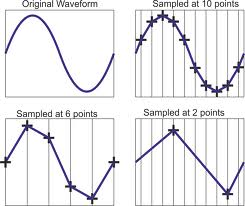
\includegraphics[scale=0.7]{../images/muestreo.png}
 \caption{Frecuencia de Muestreo.}
 \label{fig:../images/muestreo.png}
 \end{figure}

\noindent\textbf{¿Qué es la Profundidad de bit?}\\
Resolución de captura de una señal de audio en relación a la amplitud (volumen). La Profundidad de Bits determina el rango dinámico de una señal de audio, es decir, determina el máximo y mínimo de decibelios que una señal puede tener al ser grabada.\\

\noindent\textbf{¿Qué es la Calidad/Fidelidad del sonido?}\\
Para los sistemas de audio, esta medida va ha estar determinada por el número de bits por muestra y la tasa de muestreo[Figura 16].\\

 \begin{figure}[h]
 \centering
 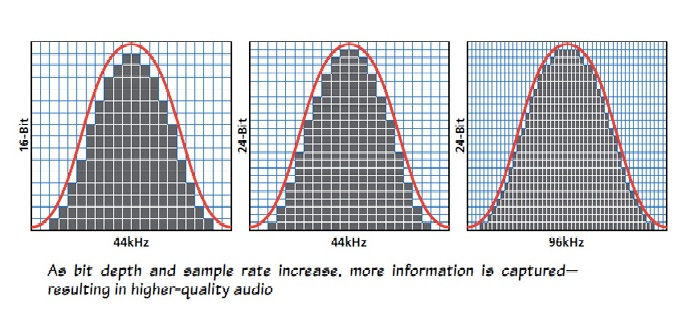
\includegraphics[scale=0.6]{../images/fidelidad_sonido.png}
 \caption{Calidad/Fidelidad del sonido.}
 \label{fig:../images/fidelidad_sonido.png}
 \end{figure}

\noindent\textbf{¿Qué es la FFT o transformada de Fourier?}\\
La transformada de Fourier se utiliza para conocer las características frecuenciales de las señales y el comportamiento de los sistemas lineales ante estas señales [Figura 17].\\

 \begin{figure}[h]
 \centering
 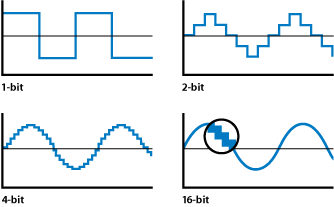
\includegraphics[scale=0.6]{../images/fouries.png}
 \caption{Seguir.}
 \label{fig:../images/fouries.png}
 \end{figure}

La interfaz AnalyserNode representa un nodo capaz de proporcionar la frecuencia en tiempo real y análisis de la información de dominio en el tiempo. Es un AudioNode que pasa el flujo de audio sin cambios desde la entrada a la salida. El nodo funciona incluso si la salida no está conectada.

Propiedades nodo AnalyserNode (hereda las propiedades del padre AudioNode): 

AnalyserNode.fftSize

Es un número sin signo que representa el tamaño de la transformada rápida de Fourier que se utilizará para determinar el dominio de la frecuencia. Debe ser una potencia distinta de cero,  en intervalos de a  2,  entre 32 y 2.048.  Su valor por defecto es 2048. Si no es una potencia de 2, o se encuentra fuera del rango especificado, saltaría una excepción.

AnalyserNode.frequencyBinCount (sólo lectura)

Contiene la mitad del tamaño de la FFT.

Métodos nodo AnalyserNode (hereda los métodos del padre AudioNode):

Analyser.getByteFrequencyData()

Copia los datos de frecuencia actual en la matriz. Si la matriz tiene menos elementos que el frequencyBinCount, el exceso de elementos se borra. Si tiene más elementos de los necesarios, se ignora el exceso de elementos.

Analyser.getByteTimeDomainData()

Copia la forma de onda actual, o el dominio del tiempo. Si la matriz tiene menos elementos que el fftSize, el exceso de elementos se borra. Si tiene más elementos de los necesarios, se ignora el exceso de elementos.



\subsection{Flujo de trabajo de la aplicación}
\label{sec:flujo}
La aplicacion se encontrara dentro de un bucle infinito desde el comienzo de la misma hasta su final. El proceso será el siguiente:
\begin{enumerate}
 \item Inicio de la iteración.
 \item El mundo actualiza su tiempo y llama a cada nanobot.
 \item Cada nanobot comprueba si recibe algún estímulo externo, si lo recibe almacena la información de dichos estímulos.
 \item Se actualiza las variables según dichos estímulos para cada nanobot.
 \item Cada nanobot realiza los cálculos para llevar a cabo los comportamientos activos según las variables actuales, para terminar devolviendo una nueva aceleración.
 \item Se calcula la velocidad final para cada nanobot según la aceleración, para poder determinar la nueva posición.
 \item Se pinta el mundo y todos los nanobots en pantalla según la posición recién calculada.
 \item Termina la iteración y vuelve a empezar el bucle.
\end{enumerate}

 





